\documentclass[12pt]{article}\usepackage[]{graphicx}\usepackage[]{color}
% maxwidth is the original width if it is less than linewidth
% otherwise use linewidth (to make sure the graphics do not exceed the margin)
\makeatletter
\def\maxwidth{ %
  \ifdim\Gin@nat@width>\linewidth
    \linewidth
  \else
    \Gin@nat@width
  \fi
}
\makeatother

\definecolor{fgcolor}{rgb}{0.345, 0.345, 0.345}
\newcommand{\hlnum}[1]{\textcolor[rgb]{0.686,0.059,0.569}{#1}}%
\newcommand{\hlstr}[1]{\textcolor[rgb]{0.192,0.494,0.8}{#1}}%
\newcommand{\hlcom}[1]{\textcolor[rgb]{0.678,0.584,0.686}{\textit{#1}}}%
\newcommand{\hlopt}[1]{\textcolor[rgb]{0,0,0}{#1}}%
\newcommand{\hlstd}[1]{\textcolor[rgb]{0.345,0.345,0.345}{#1}}%
\newcommand{\hlkwa}[1]{\textcolor[rgb]{0.161,0.373,0.58}{\textbf{#1}}}%
\newcommand{\hlkwb}[1]{\textcolor[rgb]{0.69,0.353,0.396}{#1}}%
\newcommand{\hlkwc}[1]{\textcolor[rgb]{0.333,0.667,0.333}{#1}}%
\newcommand{\hlkwd}[1]{\textcolor[rgb]{0.737,0.353,0.396}{\textbf{#1}}}%
\let\hlipl\hlkwb

\usepackage{framed}
\makeatletter
\newenvironment{kframe}{%
 \def\at@end@of@kframe{}%
 \ifinner\ifhmode%
  \def\at@end@of@kframe{\end{minipage}}%
  \begin{minipage}{\columnwidth}%
 \fi\fi%
 \def\FrameCommand##1{\hskip\@totalleftmargin \hskip-\fboxsep
 \colorbox{shadecolor}{##1}\hskip-\fboxsep
     % There is no \\@totalrightmargin, so:
     \hskip-\linewidth \hskip-\@totalleftmargin \hskip\columnwidth}%
 \MakeFramed {\advance\hsize-\width
   \@totalleftmargin\z@ \linewidth\hsize
   \@setminipage}}%
 {\par\unskip\endMakeFramed%
 \at@end@of@kframe}
\makeatother

\definecolor{shadecolor}{rgb}{.97, .97, .97}
\definecolor{messagecolor}{rgb}{0, 0, 0}
\definecolor{warningcolor}{rgb}{1, 0, 1}
\definecolor{errorcolor}{rgb}{1, 0, 0}
\newenvironment{knitrout}{}{} % an empty environment to be redefined in TeX

\usepackage{alltt}
 
\usepackage[margin=1in]{geometry}
\usepackage{amsmath,amsthm,amssymb, mathtools}
\usepackage[T1]{fontenc}
\usepackage{lmodern}
\usepackage{fixltx2e}
\usepackage[shortlabels]{enumitem}
 
\newcommand{\N}{\mathbb{N}}
\newcommand{\R}{\mathbb{R}}
\newcommand{\Z}{\mathbb{Z}}
\newcommand{\Q}{\mathbb{Q}}

\newenvironment{theorem}[2][Theorem]{\begin{trivlist}
\item[\hskip \labelsep {\bfseries #1}\hskip \labelsep {\bfseries #2.}]}{\end{trivlist}}
\newenvironment{lemma}[2][Lemma]{\begin{trivlist}
\item[\hskip \labelsep {\bfseries #1}\hskip \labelsep {\bfseries #2.}]}{\end{trivlist}}
\newenvironment{exercise}[2][Exercise]{\begin{trivlist}
\item[\hskip \labelsep {\bfseries #1}\hskip \labelsep {\bfseries #2.}]}{\end{trivlist}}
\newenvironment{problem}[2][Problem]{\begin{trivlist}
\item[\hskip \labelsep {\bfseries #1}\hskip \labelsep {\bfseries #2.}]}{\end{trivlist}}
\newenvironment{question}[2][Question]{\begin{trivlist}
\item[\hskip \labelsep {\bfseries #1}\hskip \labelsep {\bfseries #2.}]}{\end{trivlist}}
\newenvironment{corollary}[2][Corollary]{\begin{trivlist}
\item[\hskip \labelsep {\bfseries #1}\hskip \labelsep {\bfseries #2.}]}{\end{trivlist}}
\newcommand{\textfrac}[2]{\dfrac{\text{#1}}{\text{#2}}}
\IfFileExists{upquote.sty}{\usepackage{upquote}}{}
\begin{document}

\title{Ch. 7 - Moving Beyond Linearity}

\author{Chris Hayduk}
\date{\today}

\maketitle



\section{Polynomial Regression and Step Functions}

Polynomial regression and step functions both exist to give a more flexible fit than standard linear regression will allow. Polynomial regression works by creating new variables out of powers of the initial prediction variable. For example, if the initial predictor is $x$, we may use $x, x^2$, and $x^3$ as our three predictors if we wish to use a cubic fit. On the other than, step functions work by cutitng the data up into bins and then fitting constant functions on each of these bins.\\

We start here by fitting a degree 4 polynomial with the \texttt{lm()} function.

\begin{knitrout}
\definecolor{shadecolor}{rgb}{0.969, 0.969, 0.969}\color{fgcolor}\begin{kframe}
\begin{alltt}
\hlkwd{data}\hlstd{(Wage)}
\hlkwd{attach}\hlstd{(Wage)}
\hlstd{fit}\hlkwb{=}\hlkwd{lm}\hlstd{(wage}\hlopt{~}\hlkwd{poly}\hlstd{(age,}\hlnum{4}\hlstd{),} \hlkwc{data}\hlstd{=Wage)}
\hlkwd{coef}\hlstd{(}\hlkwd{summary}\hlstd{(fit))}
\end{alltt}
\begin{verbatim}
##                 Estimate Std. Error    t value     Pr(>|t|)
## (Intercept)    111.70361  0.7287409 153.283015 0.000000e+00
## poly(age, 4)1  447.06785 39.9147851  11.200558 1.484604e-28
## poly(age, 4)2 -478.31581 39.9147851 -11.983424 2.355831e-32
## poly(age, 4)3  125.52169 39.9147851   3.144742 1.678622e-03
## poly(age, 4)4  -77.91118 39.9147851  -1.951938 5.103865e-02
\end{verbatim}
\end{kframe}
\end{knitrout}

The \texttt{poly()} function used above allows us to avoid writing out a long equation by hand. However, by default it returns a matrix whose columns are a basis of orthogonal polynomials. That is, each column is a linear combination of the variables $\text{age}, \text{age}^2, \text{age}^3$, and $\text{age}^4$. While the choice of basis will not affect the fitted values, we may want to use $\text{age}, \text{age}^2, \text{age}^3$, and $\text{age}^4$ directly. We can do this by setting \texttt{raw=TRUE} in the arguments for the function \texttt{poly()}.

\begin{knitrout}
\definecolor{shadecolor}{rgb}{0.969, 0.969, 0.969}\color{fgcolor}\begin{kframe}
\begin{alltt}
\hlstd{fit2}\hlkwb{=}\hlkwd{lm}\hlstd{(wage}\hlopt{~}\hlkwd{poly}\hlstd{(age,}\hlnum{4}\hlstd{,}\hlkwc{raw}\hlstd{=T),}\hlkwc{data}\hlstd{=Wage)}
\hlkwd{coef}\hlstd{(}\hlkwd{summary}\hlstd{(fit2))}
\end{alltt}
\begin{verbatim}
##                             Estimate   Std. Error   t value     Pr(>|t|)
## (Intercept)            -1.841542e+02 6.004038e+01 -3.067172 0.0021802539
## poly(age, 4, raw = T)1  2.124552e+01 5.886748e+00  3.609042 0.0003123618
## poly(age, 4, raw = T)2 -5.638593e-01 2.061083e-01 -2.735743 0.0062606446
## poly(age, 4, raw = T)3  6.810688e-03 3.065931e-03  2.221409 0.0263977518
## poly(age, 4, raw = T)4 -3.203830e-05 1.641359e-05 -1.951938 0.0510386498
\end{verbatim}
\end{kframe}
\end{knitrout}

There are several other equivalent was of fitting this model in R. For example,

\begin{knitrout}
\definecolor{shadecolor}{rgb}{0.969, 0.969, 0.969}\color{fgcolor}\begin{kframe}
\begin{alltt}
\hlstd{fit2a} \hlkwb{=} \hlkwd{lm}\hlstd{(wage}\hlopt{~}\hlstd{age}\hlopt{+}\hlkwd{I}\hlstd{(age}\hlopt{^}\hlnum{2}\hlstd{)}\hlopt{+}\hlkwd{I}\hlstd{(age}\hlopt{^}\hlnum{3}\hlstd{)}\hlopt{+}\hlkwd{I}\hlstd{(age}\hlopt{^}\hlnum{4}\hlstd{),} \hlkwc{data}\hlstd{=Wage)}
\hlkwd{coef}\hlstd{(fit2a)}
\end{alltt}
\begin{verbatim}
##   (Intercept)           age      I(age^2)      I(age^3)      I(age^4) 
## -1.841542e+02  2.124552e+01 -5.638593e-01  6.810688e-03 -3.203830e-05
\end{verbatim}
\end{kframe}
\end{knitrout}

and,

\begin{knitrout}
\definecolor{shadecolor}{rgb}{0.969, 0.969, 0.969}\color{fgcolor}\begin{kframe}
\begin{alltt}
\hlstd{fit2b} \hlkwb{=} \hlkwd{lm}\hlstd{(wage}\hlopt{~}\hlkwd{cbind}\hlstd{(age, age}\hlopt{^}\hlnum{2}\hlstd{, age}\hlopt{^}\hlnum{3}\hlstd{, age}\hlopt{^}\hlnum{4}\hlstd{),} \hlkwc{data} \hlstd{= Wage)}
\end{alltt}
\end{kframe}
\end{knitrout}

We now create a grid of values for \texttt{age} at which we want predictions, and then call the generic \texttt{predict()} function, specifying that we want standard errors as well.

\begin{knitrout}
\definecolor{shadecolor}{rgb}{0.969, 0.969, 0.969}\color{fgcolor}\begin{kframe}
\begin{alltt}
\hlstd{agelims}\hlkwb{=}\hlkwd{range}\hlstd{(age)}
\hlstd{age.grid}\hlkwb{=}\hlkwd{seq}\hlstd{(}\hlkwc{from}\hlstd{=agelims[}\hlnum{1}\hlstd{],} \hlkwc{to} \hlstd{= agelims[}\hlnum{2}\hlstd{])}
\hlstd{preds}\hlkwb{=}\hlkwd{predict}\hlstd{(fit,} \hlkwc{newdata}\hlstd{=}\hlkwd{list}\hlstd{(}\hlkwc{age}\hlstd{=age.grid),} \hlkwc{se}\hlstd{=}\hlnum{TRUE}\hlstd{)}
\hlstd{se.bands} \hlkwb{=} \hlkwd{cbind}\hlstd{(preds}\hlopt{$}\hlstd{fit}\hlopt{+}\hlnum{2}\hlopt{*}\hlstd{preds}\hlopt{$}\hlstd{se.fit, preds}\hlopt{$}\hlstd{fit}\hlopt{-}\hlnum{2}\hlopt{*}\hlstd{preds}\hlopt{$}\hlstd{se.fit)}
\end{alltt}
\end{kframe}
\end{knitrout}

The above code creates our grid of age values, gets predictions for each value in the grid, and then sets the standard error bars at 95\% confidence (two times the standard error plus/minus the prediction). Finally, let us plot the data and add the fit from the degree-4 polynomial.

\begin{knitrout}
\definecolor{shadecolor}{rgb}{0.969, 0.969, 0.969}\color{fgcolor}\begin{kframe}
\begin{alltt}
\hlkwd{par}\hlstd{(}\hlkwc{mfrow}\hlstd{=}\hlkwd{c}\hlstd{(}\hlnum{1}\hlstd{,}\hlnum{1}\hlstd{),} \hlkwc{mar}\hlstd{=}\hlkwd{c}\hlstd{(}\hlnum{4.5}\hlstd{,}\hlnum{4.5}\hlstd{,}\hlnum{1}\hlstd{,}\hlnum{1}\hlstd{),} \hlkwc{oma}\hlstd{=}\hlkwd{c}\hlstd{(}\hlnum{0}\hlstd{,}\hlnum{0}\hlstd{,}\hlnum{4}\hlstd{,}\hlnum{0}\hlstd{))}
\hlkwd{plot}\hlstd{(age, wage,} \hlkwc{xlim}\hlstd{=agelims,} \hlkwc{cex}\hlstd{=}\hlnum{.5}\hlstd{,} \hlkwc{col}\hlstd{=}\hlstr{"darkgrey"}\hlstd{)}
\hlkwd{title}\hlstd{(}\hlstr{"Degree-4 Polynomial"}\hlstd{,} \hlkwc{outer}\hlstd{=T)}
\hlkwd{lines}\hlstd{(age.grid, preds}\hlopt{$}\hlstd{fit,} \hlkwc{lwd}\hlstd{=}\hlnum{2}\hlstd{,} \hlkwc{col}\hlstd{=}\hlstr{"blue"}\hlstd{)}
\hlkwd{matlines}\hlstd{(age.grid, se.bands,} \hlkwc{lwd}\hlstd{=}\hlnum{1}\hlstd{,} \hlkwc{col}\hlstd{=}\hlstr{"blue"}\hlstd{,} \hlkwc{lty}\hlstd{=}\hlnum{3}\hlstd{)}
\end{alltt}
\end{kframe}
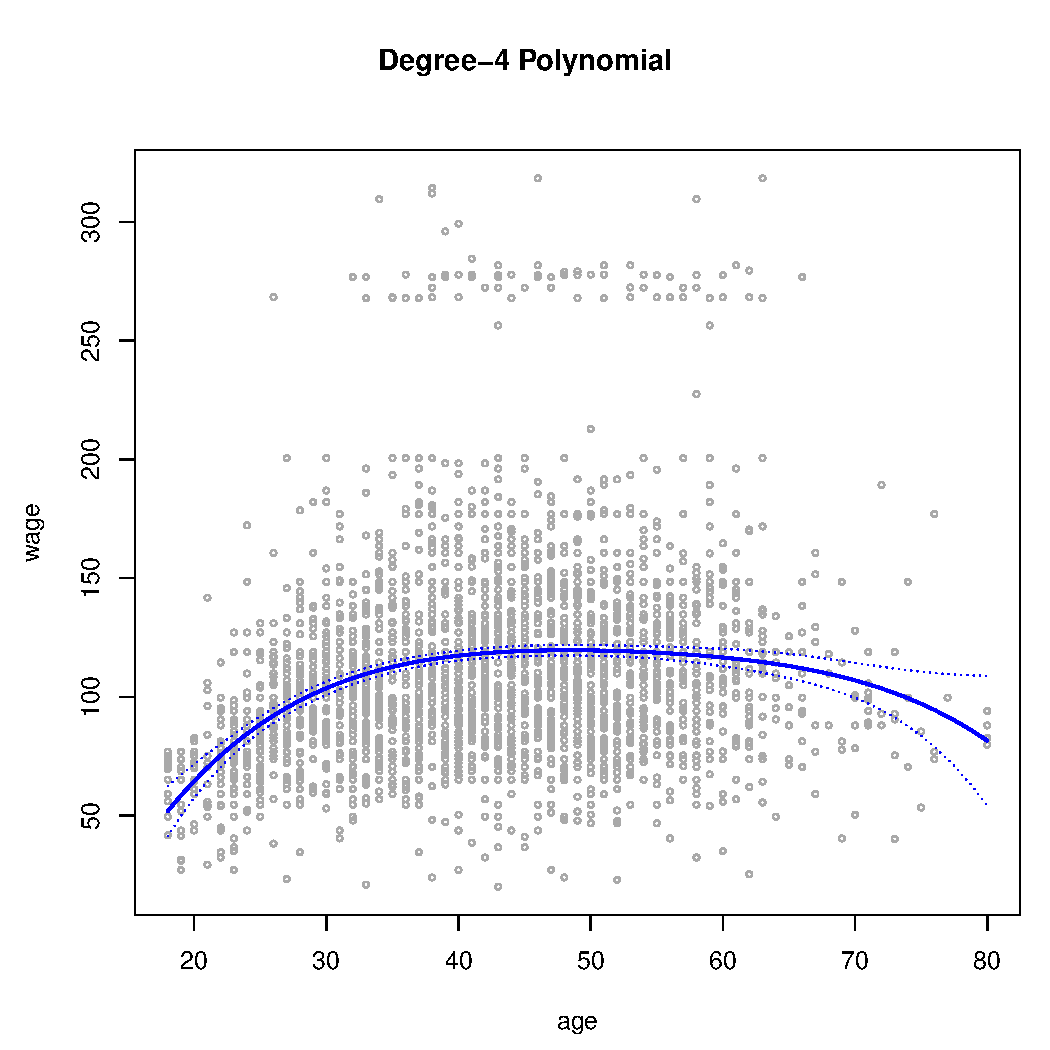
\includegraphics[width=\maxwidth]{figure/unnamed-chunk-7-1} 

\end{knitrout}

As we mentioned above, the choice of basis will not affect the fitted values of the function. We can verify this by checking the predicted values on our age grid from both types of our fitted polynomial functions:

\begin{knitrout}
\definecolor{shadecolor}{rgb}{0.969, 0.969, 0.969}\color{fgcolor}\begin{kframe}
\begin{alltt}
\hlstd{preds2} \hlkwb{=} \hlkwd{predict}\hlstd{(fit2,} \hlkwc{newdata}\hlstd{=}\hlkwd{list}\hlstd{(}\hlkwc{age}\hlstd{=age.grid),} \hlkwc{se}\hlstd{=}\hlnum{TRUE}\hlstd{)}
\hlkwd{max}\hlstd{(}\hlkwd{abs}\hlstd{(preds}\hlopt{$}\hlstd{fit}\hlopt{-}\hlstd{preds2}\hlopt{$}\hlstd{fit))}
\end{alltt}
\begin{verbatim}
## [1] 7.81597e-11
\end{verbatim}
\end{kframe}
\end{knitrout}

As we can see, the maximum of the absolute value of the difference of these two fits is extremely close to 0.\\

In practice, we will want to check several possible polynomial degrees in order to find the simplest model that provides the best fit. We will now fit models ranging from linear to degree-5 polynomials and use the \texttt{anova()} function to perform an analysis of variance in order to determine the best model. Analysis of variance (ANOVA) works by testing the null hypothesis that a model $M_1$ is sufficient to explain the data again the alternative hypothesis that a more complex model $M_2$ is required. In order to use the \texttt{anova()} function, $M_1$ and $M_2$ must be nested models. In this case, we are fitting five different models and wll sequentially compare the simpler model to the more complex model.

\begin{knitrout}
\definecolor{shadecolor}{rgb}{0.969, 0.969, 0.969}\color{fgcolor}\begin{kframe}
\begin{alltt}
\hlstd{fit.1} \hlkwb{=} \hlkwd{lm}\hlstd{(wage}\hlopt{~}\hlstd{age,} \hlkwc{data}\hlstd{=Wage)}
\hlstd{fit.2} \hlkwb{=} \hlkwd{lm}\hlstd{(wage}\hlopt{~}\hlkwd{poly}\hlstd{(age,}\hlnum{2}\hlstd{),} \hlkwc{data}\hlstd{=Wage)}
\hlstd{fit.3} \hlkwb{=} \hlkwd{lm}\hlstd{(wage}\hlopt{~}\hlkwd{poly}\hlstd{(age,}\hlnum{3}\hlstd{),} \hlkwc{data}\hlstd{=Wage)}
\hlstd{fit.4} \hlkwb{=} \hlkwd{lm}\hlstd{(wage}\hlopt{~}\hlkwd{poly}\hlstd{(age,}\hlnum{4}\hlstd{),} \hlkwc{data}\hlstd{=Wage)}
\hlstd{fit.5} \hlkwb{=} \hlkwd{lm}\hlstd{(wage}\hlopt{~}\hlkwd{poly}\hlstd{(age,}\hlnum{5}\hlstd{),} \hlkwc{data}\hlstd{=Wage)}
\hlkwd{anova}\hlstd{(fit.1, fit.2, fit.3, fit.4, fit.5)}
\end{alltt}
\begin{verbatim}
## Analysis of Variance Table
## 
## Model 1: wage ~ age
## Model 2: wage ~ poly(age, 2)
## Model 3: wage ~ poly(age, 3)
## Model 4: wage ~ poly(age, 4)
## Model 5: wage ~ poly(age, 5)
##   Res.Df     RSS Df Sum of Sq        F    Pr(>F)    
## 1   2998 5022216                                    
## 2   2997 4793430  1    228786 143.5931 < 2.2e-16 ***
## 3   2996 4777674  1     15756   9.8888  0.001679 ** 
## 4   2995 4771604  1      6070   3.8098  0.051046 .  
## 5   2994 4770322  1      1283   0.8050  0.369682    
## ---
## Signif. codes:  0 '***' 0.001 '**' 0.01 '*' 0.05 '.' 0.1 ' ' 1
\end{verbatim}
\end{kframe}
\end{knitrout}

The p-value comparing the linear Model 1 to the quadratic Model 2 is essentially 0, indicating that a linear fit is not sufficient. Similarly, the p-value comparing the quadratic Model 2 to the cubic Model 3 is very low, so the quadratic fit is also insufficient. The p-value comparing the cubic model and the degree-4 polynomial is approximately 5\%, while the degree-5 polynomial seems unnecessary because its p-value is 0.37. Hence, either a cubic or quartic polynomial appears to provide a reasonable fit to the data, but lower- or higher-order models are not justified.\\

We can actually avoid using the \texttt{anova()} function since \texttt{poly()} creates orthogonal polynomials:

\begin{knitrout}
\definecolor{shadecolor}{rgb}{0.969, 0.969, 0.969}\color{fgcolor}\begin{kframe}
\begin{alltt}
\hlkwd{coef}\hlstd{(}\hlkwd{summary}\hlstd{(fit.5))}
\end{alltt}
\begin{verbatim}
##                 Estimate Std. Error     t value     Pr(>|t|)
## (Intercept)    111.70361  0.7287647 153.2780243 0.000000e+00
## poly(age, 5)1  447.06785 39.9160847  11.2001930 1.491111e-28
## poly(age, 5)2 -478.31581 39.9160847 -11.9830341 2.367734e-32
## poly(age, 5)3  125.52169 39.9160847   3.1446392 1.679213e-03
## poly(age, 5)4  -77.91118 39.9160847  -1.9518743 5.104623e-02
## poly(age, 5)5  -35.81289 39.9160847  -0.8972045 3.696820e-01
\end{verbatim}
\end{kframe}
\end{knitrout}

As you can see, the p-values aree exactly the same, and in fact the square of the t-statistics are equal to the F-statistics from the \texttt{anova()} function. However, the ANOVA method works whether or not we used orthogonal polynomials; it also works when we have other terms in the model as well. For example, we can use \texttt{anova()} to compare these three models:

\begin{knitrout}
\definecolor{shadecolor}{rgb}{0.969, 0.969, 0.969}\color{fgcolor}\begin{kframe}
\begin{alltt}
\hlstd{fit.1} \hlkwb{=} \hlkwd{lm}\hlstd{(wage}\hlopt{~}\hlstd{education}\hlopt{+}\hlstd{age,} \hlkwc{data}\hlstd{=Wage)}
\hlstd{fit.2} \hlkwb{=} \hlkwd{lm}\hlstd{(wage}\hlopt{~}\hlstd{education} \hlopt{+} \hlkwd{poly}\hlstd{(age,}\hlnum{2}\hlstd{),} \hlkwc{data}\hlstd{=Wage)}
\hlstd{fit.3} \hlkwb{=} \hlkwd{lm}\hlstd{(wage}\hlopt{~}\hlstd{education}\hlopt{+}\hlkwd{poly}\hlstd{(age,}\hlnum{3}\hlstd{),} \hlkwc{data}\hlstd{=Wage)}
\hlkwd{anova}\hlstd{(fit.1, fit.2, fit.3)}
\end{alltt}
\begin{verbatim}
## Analysis of Variance Table
## 
## Model 1: wage ~ education + age
## Model 2: wage ~ education + poly(age, 2)
## Model 3: wage ~ education + poly(age, 3)
##   Res.Df     RSS Df Sum of Sq        F Pr(>F)    
## 1   2994 3867992                                 
## 2   2993 3725395  1    142597 114.6969 <2e-16 ***
## 3   2992 3719809  1      5587   4.4936 0.0341 *  
## ---
## Signif. codes:  0 '***' 0.001 '**' 0.01 '*' 0.05 '.' 0.1 ' ' 1
\end{verbatim}
\end{kframe}
\end{knitrout}

As an alternative to using ANOVA, we could also choose the polynomial degree using cross-validation.\\

Now let us consider the task of predicting whether an individual earns more than \$250,000 per year. We proceed much as before, except that first we create the appropriate response vector, and then apply the \texttt{glm()} function using \texttt{family=''binomial``} in order to fit a polynomial logistic regression model.

\begin{knitrout}
\definecolor{shadecolor}{rgb}{0.969, 0.969, 0.969}\color{fgcolor}\begin{kframe}
\begin{alltt}
\hlstd{fit} \hlkwb{=} \hlkwd{glm}\hlstd{(}\hlkwd{I}\hlstd{(wage}\hlopt{>}\hlnum{250}\hlstd{)} \hlopt{~} \hlkwd{poly}\hlstd{(age,}\hlnum{4}\hlstd{),} \hlkwc{data} \hlstd{= Wage,} \hlkwc{family} \hlstd{= binomial)}
\end{alltt}
\end{kframe}
\end{knitrout}

We are using the wrapper \texttt{I()} to create the binary response variable on the fly. The expression \texttt{wage>250} evaluates to a logical vairable containing \texttt{TRUEs} and \texttt{FALSEs}, which \texttt{glm()} coerces to binary by setting \texttt{TRUEs} to $1$ and \texttt{FALSEs} to $0$.\\

We now use the \texttt{predict()} function to make our predictions,
\begin{knitrout}
\definecolor{shadecolor}{rgb}{0.969, 0.969, 0.969}\color{fgcolor}\begin{kframe}
\begin{alltt}
\hlstd{preds}\hlkwb{=}\hlkwd{predict}\hlstd{(fit,} \hlkwc{newdata}\hlstd{=}\hlkwd{list}\hlstd{(}\hlkwc{age}\hlstd{=age.grid),}\hlkwc{se}\hlstd{=T)}
\end{alltt}
\end{kframe}
\end{knitrout}

Confidence intervals in this scenario are a bit more involved than they were in the linear regression case. Our predictions are for the \textit{logit}. That is, we have fit a model of the form $$\log \left(\frac{\text{Pr}(Y=1|X)}{1 - \text{Pr}(Y=1|X)}\right) = X\beta$$, and the predictions given are of the form $X\hat{\beta}$. The standard errors given are also of this form. In order to obtain confidence intervals for $\text{Pr}(Y=1|X)$, we use the transformation $$\text{Pr}(Y=1|X) = \frac{\exp(X\beta)}{1 + \exp(X\beta)}$$

\begin{knitrout}
\definecolor{shadecolor}{rgb}{0.969, 0.969, 0.969}\color{fgcolor}\begin{kframe}
\begin{alltt}
\hlstd{pfit} \hlkwb{=} \hlkwd{exp}\hlstd{(preds}\hlopt{$}\hlstd{fit)}\hlopt{/}\hlstd{(}\hlnum{1}\hlopt{+}\hlkwd{exp}\hlstd{(preds}\hlopt{$}\hlstd{fit))}
\hlstd{se.bands.logit} \hlkwb{=} \hlkwd{cbind}\hlstd{(preds}\hlopt{$}\hlstd{fit}\hlopt{+}\hlnum{2}\hlopt{*}\hlstd{preds}\hlopt{$}\hlstd{se.fit, preds}\hlopt{$}\hlstd{fit}\hlopt{-}\hlnum{2}\hlopt{*}\hlstd{preds}\hlopt{$}\hlstd{se.fit)}
\hlstd{se.bands} \hlkwb{=} \hlkwd{exp}\hlstd{(se.bands.logit)}\hlopt{/}\hlstd{(}\hlnum{1}\hlopt{+}\hlkwd{exp}\hlstd{(se.bands.logit))}
\end{alltt}
\end{kframe}
\end{knitrout}

However, the corresponding confidence intervals would not have been sensible because we would end up with negative probabilities! Finally, the right-hand plot from Figure 7.1 was made as follows:

\begin{knitrout}
\definecolor{shadecolor}{rgb}{0.969, 0.969, 0.969}\color{fgcolor}\begin{kframe}
\begin{alltt}
\hlkwd{plot}\hlstd{(age,}\hlkwd{I}\hlstd{(wage}\hlopt{>}\hlnum{250}\hlstd{),} \hlkwc{xlim}\hlstd{=agelims,} \hlkwc{type}\hlstd{=}\hlstr{"n"}\hlstd{,} \hlkwc{ylim}\hlstd{=}\hlkwd{c}\hlstd{(}\hlnum{0}\hlstd{,}\hlnum{0.2}\hlstd{))}
\hlkwd{points}\hlstd{(}\hlkwd{jitter}\hlstd{(age),} \hlkwd{I}\hlstd{((wage}\hlopt{>}\hlnum{250}\hlstd{)}\hlopt{/}\hlnum{5}\hlstd{),} \hlkwc{cex}\hlstd{=}\hlnum{.5}\hlstd{,} \hlkwc{pch}\hlstd{=}\hlstr{"|"}\hlstd{,} \hlkwc{col}\hlstd{=}\hlstr{"darkgrey"}\hlstd{)}
\hlkwd{lines}\hlstd{(age.grid, pfit,} \hlkwc{lwd}\hlstd{=}\hlnum{2}\hlstd{,} \hlkwc{col}\hlstd{=}\hlstr{"blue"}\hlstd{)}
\hlkwd{matlines}\hlstd{(age.grid, se.bands,} \hlkwc{lwd}\hlstd{=}\hlnum{1}\hlstd{,} \hlkwc{col}\hlstd{=}\hlstr{"blue"}\hlstd{,} \hlkwc{lty}\hlstd{=}\hlnum{3}\hlstd{)}
\end{alltt}
\end{kframe}
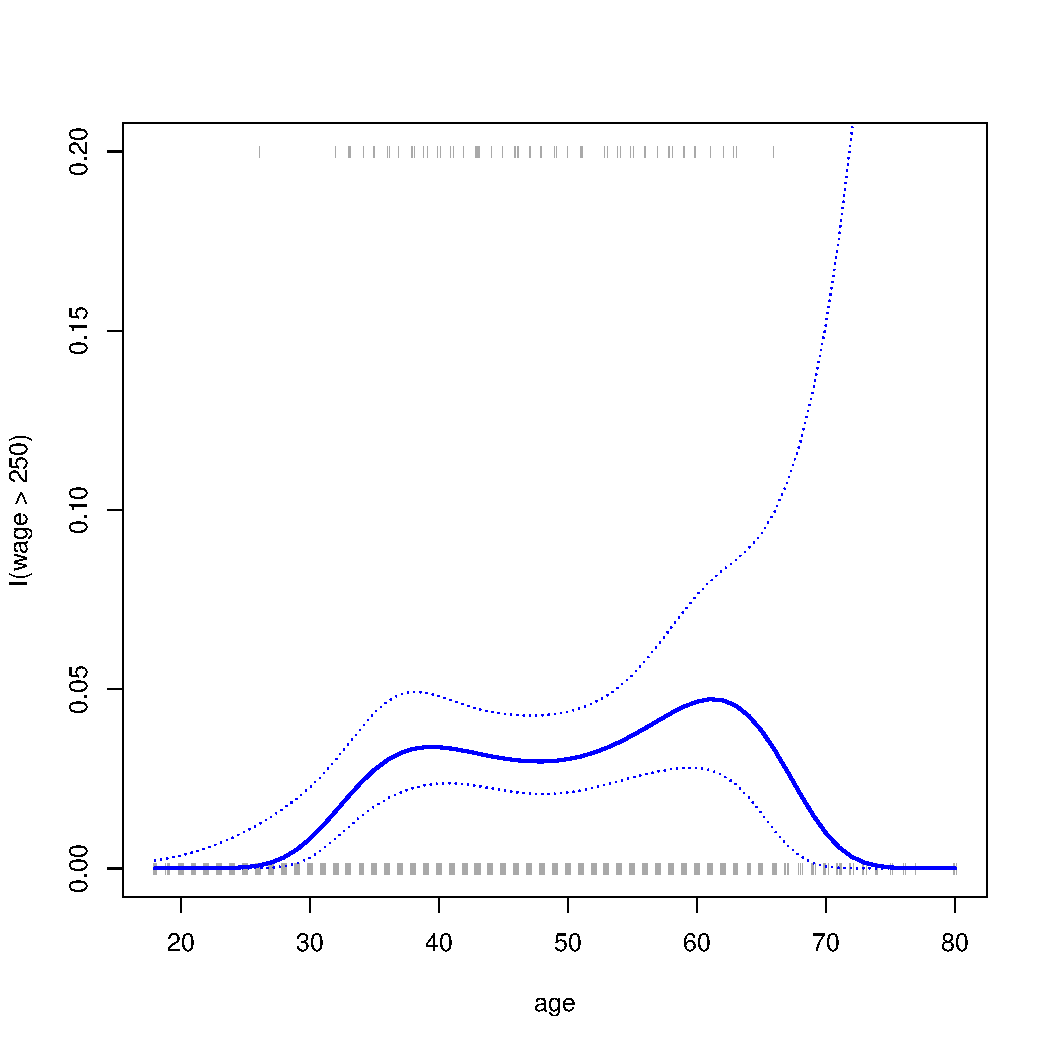
\includegraphics[width=\maxwidth]{figure/unnamed-chunk-15-1} 

\end{knitrout}

In order to fit a step function, as discussed in Section 7.2, we use the \texttt{cut()} function.

\begin{knitrout}
\definecolor{shadecolor}{rgb}{0.969, 0.969, 0.969}\color{fgcolor}\begin{kframe}
\begin{alltt}
\hlkwd{table}\hlstd{(}\hlkwd{cut}\hlstd{(age,}\hlnum{4}\hlstd{))}
\end{alltt}
\begin{verbatim}
## 
## (17.9,33.5]   (33.5,49]   (49,64.5] (64.5,80.1] 
##         750        1399         779          72
\end{verbatim}
\begin{alltt}
\hlstd{fit}\hlkwb{=}\hlkwd{lm}\hlstd{(wage}\hlopt{~}\hlkwd{cut}\hlstd{(age,}\hlnum{4}\hlstd{),} \hlkwc{data} \hlstd{= Wage)}
\hlkwd{coef}\hlstd{(}\hlkwd{summary}\hlstd{(fit))}
\end{alltt}
\begin{verbatim}
##                         Estimate Std. Error   t value     Pr(>|t|)
## (Intercept)            94.158392   1.476069 63.789970 0.000000e+00
## cut(age, 4)(33.5,49]   24.053491   1.829431 13.148074 1.982315e-38
## cut(age, 4)(49,64.5]   23.664559   2.067958 11.443444 1.040750e-29
## cut(age, 4)(64.5,80.1]  7.640592   4.987424  1.531972 1.256350e-01
\end{verbatim}
\end{kframe}
\end{knitrout}

Here \texttt{cut()} automatically picked the cutpoints at 33.5, 49, and 64.5 years of age. The function \texttt{cut()} returns an ordered categorical variable; the \texttt{lm()} function then creates a set of dummy variables for use in the regression. The \texttt{age<33.5} category is left out, so the intercept coefficient of \$94,160 can be interpreted as the average salary for those under 33.5 years of age, and the other coefficients can be interpreted as the average additional salary for those in the other age groups.\\

We can produce predictions and plots just as we did in the case of the polynomial fit:
\begin{knitrout}
\definecolor{shadecolor}{rgb}{0.969, 0.969, 0.969}\color{fgcolor}\begin{kframe}
\begin{alltt}
\hlstd{preds}\hlkwb{=}\hlkwd{predict}\hlstd{(fit,} \hlkwc{newdata}\hlstd{=}\hlkwd{list}\hlstd{(}\hlkwc{age}\hlstd{=age.grid),} \hlkwc{se}\hlstd{=}\hlnum{TRUE}\hlstd{)}
\hlstd{se.bands} \hlkwb{=} \hlkwd{cbind}\hlstd{(preds}\hlopt{$}\hlstd{fit}\hlopt{+}\hlnum{2}\hlopt{*}\hlstd{preds}\hlopt{$}\hlstd{se.fit, preds}\hlopt{$}\hlstd{fit}\hlopt{-}\hlnum{2}\hlopt{*}\hlstd{preds}\hlopt{$}\hlstd{se.fit)}

\hlkwd{plot}\hlstd{(age, wage,} \hlkwc{xlim}\hlstd{=agelims,} \hlkwc{cex}\hlstd{=}\hlnum{.5}\hlstd{,} \hlkwc{col}\hlstd{=}\hlstr{"darkgrey"}\hlstd{)}
\hlkwd{title}\hlstd{(}\hlstr{"Step Function"}\hlstd{,} \hlkwc{outer}\hlstd{=T)}
\hlkwd{lines}\hlstd{(age.grid, preds}\hlopt{$}\hlstd{fit,} \hlkwc{lwd}\hlstd{=}\hlnum{2}\hlstd{,} \hlkwc{col}\hlstd{=}\hlstr{"blue"}\hlstd{)}
\hlkwd{matlines}\hlstd{(age.grid, se.bands,} \hlkwc{lwd}\hlstd{=}\hlnum{1}\hlstd{,} \hlkwc{col}\hlstd{=}\hlstr{"blue"}\hlstd{,} \hlkwc{lty}\hlstd{=}\hlnum{3}\hlstd{)}
\end{alltt}
\end{kframe}
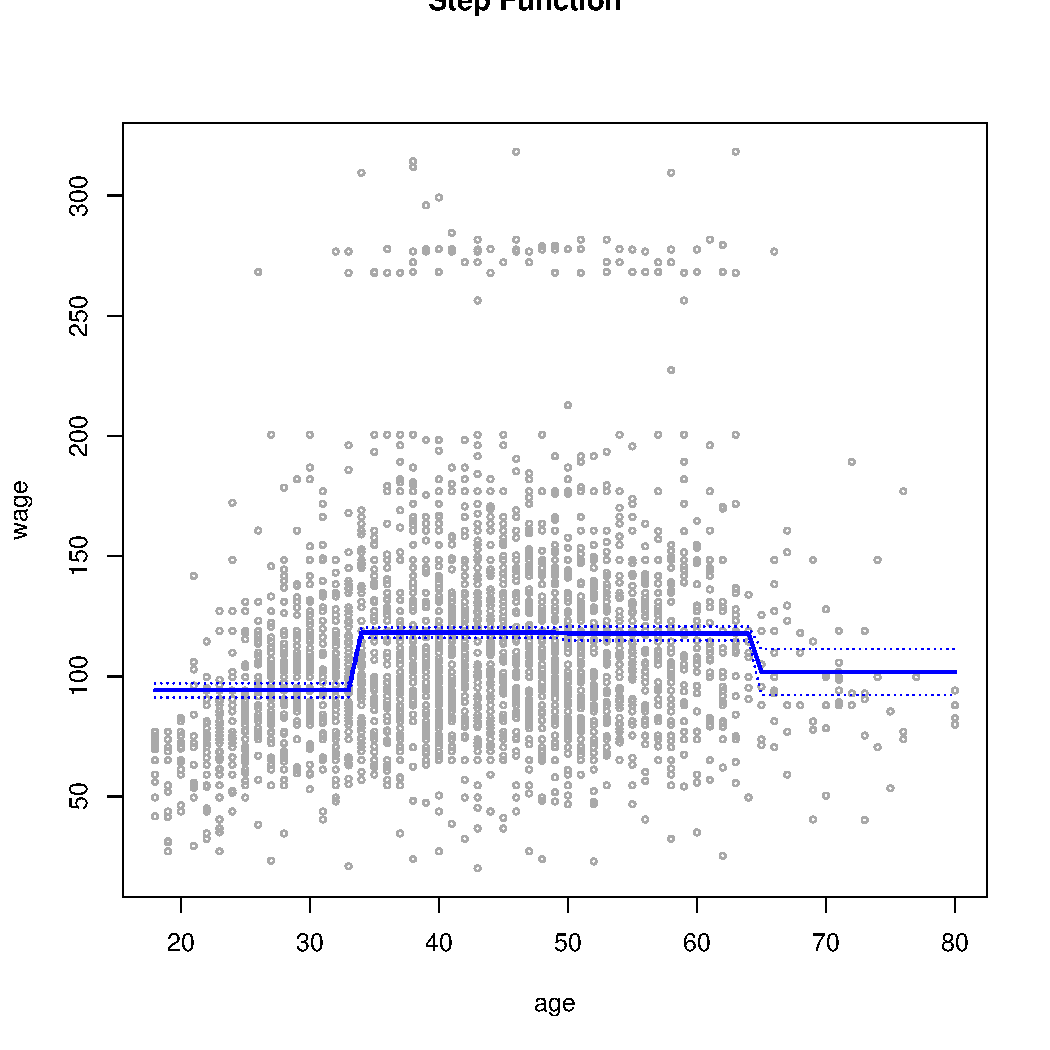
\includegraphics[width=\maxwidth]{figure/unnamed-chunk-17-1} 

\end{knitrout}

\newpage
\section{Splines}

This section covers regression splines, which is a generalization of the step function we computed in the previous section. Instead of fitting constant functions to each cut of the data, we will now fit polynomials. We generally require that these degree $n$ polynomials have continuous $n-1$st derivative at the boundaries of each cut, giving us a very smooth fit to the data.\\

In order to fit regression splines in \texttt{R}, we use the \texttt{splines} library. In Section 7.4, we saw that regression splines can be fit by constructing an appropriate matrix of basis functions. The \texttt{bs()} function generates the entire matrix of basis functions for splines with the specified set of knots. By default, cubic splines are produced (ie. the polynomials are degree $3$). Fitting \texttt{wage} to \texttt{age} using a regression spline is simple:

\begin{knitrout}
\definecolor{shadecolor}{rgb}{0.969, 0.969, 0.969}\color{fgcolor}\begin{kframe}
\begin{alltt}
\hlstd{fit}\hlkwb{=}\hlkwd{lm}\hlstd{(wage}\hlopt{~}\hlkwd{bs}\hlstd{(age,} \hlkwc{knots}\hlstd{=}\hlkwd{c}\hlstd{(}\hlnum{25}\hlstd{,}\hlnum{40}\hlstd{,}\hlnum{60}\hlstd{)),}\hlkwc{data} \hlstd{= Wage)}
\hlstd{pred} \hlkwb{=} \hlkwd{predict}\hlstd{(fit,} \hlkwc{newdata}\hlstd{=}\hlkwd{list}\hlstd{(}\hlkwc{age}\hlstd{=age.grid),}\hlkwc{se}\hlstd{=T)}
\hlkwd{plot}\hlstd{(age, wage,} \hlkwc{col}\hlstd{=}\hlstr{"gray"}\hlstd{)}
\hlkwd{lines}\hlstd{(age.grid, pred}\hlopt{$}\hlstd{fit,} \hlkwc{lwd}\hlstd{=}\hlnum{2}\hlstd{)}
\hlkwd{lines}\hlstd{(age.grid, pred}\hlopt{$}\hlstd{fit}\hlopt{+}\hlnum{2}\hlopt{*}\hlstd{pred}\hlopt{$}\hlstd{se,} \hlkwc{lty}\hlstd{=}\hlstr{"dashed"}\hlstd{)}
\hlkwd{lines}\hlstd{(age.grid, pred}\hlopt{$}\hlstd{fit}\hlopt{-}\hlnum{2}\hlopt{*}\hlstd{pred}\hlopt{$}\hlstd{se,} \hlkwc{lty}\hlstd{=}\hlstr{"dashed"}\hlstd{)}
\end{alltt}
\end{kframe}
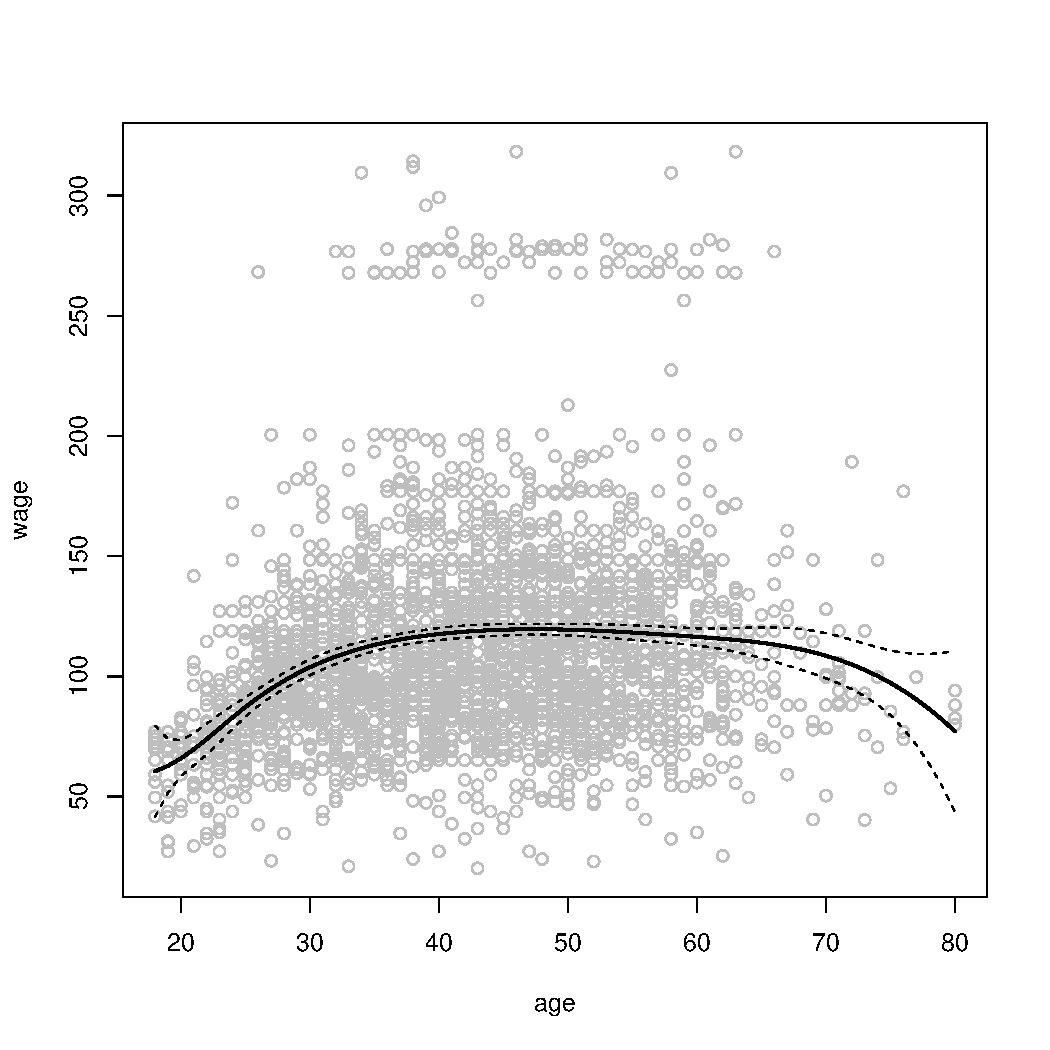
\includegraphics[width=\maxwidth]{figure/unnamed-chunk-18-1} 

\end{knitrout}

Here we have prespecified knots at ages 25, 40, and 60. This produces a spline with six basis functions. (Recall that a cubic spline with three knots has seven degrees of freedom; these degrees of freedom are used.) We could also use the \texttt{df} option to produce a spline with knots at uniform quantiles of the data.

\begin{knitrout}
\definecolor{shadecolor}{rgb}{0.969, 0.969, 0.969}\color{fgcolor}\begin{kframe}
\begin{alltt}
\hlkwd{dim}\hlstd{(}\hlkwd{bs}\hlstd{(age,} \hlkwc{knots}\hlstd{=}\hlkwd{c}\hlstd{(}\hlnum{25}\hlstd{,}\hlnum{40}\hlstd{,}\hlnum{60}\hlstd{)))}
\end{alltt}
\begin{verbatim}
## [1] 3000    6
\end{verbatim}
\begin{alltt}
\hlkwd{dim}\hlstd{(}\hlkwd{bs}\hlstd{(age,}\hlkwc{df}\hlstd{=}\hlnum{6}\hlstd{))}
\end{alltt}
\begin{verbatim}
## [1] 3000    6
\end{verbatim}
\begin{alltt}
\hlkwd{attr}\hlstd{(}\hlkwd{bs}\hlstd{(age,} \hlkwc{df}\hlstd{=}\hlnum{6}\hlstd{),}\hlstr{"knots"}\hlstd{)}
\end{alltt}
\begin{verbatim}
##   25%   50%   75% 
## 33.75 42.00 51.00
\end{verbatim}
\end{kframe}
\end{knitrout}

In this case \texttt{R} chooses knots at ages $33.8, 42.0$, and $51.0$, which correspond to the $25$th, $50$th, and $75$th percentiles of \texttt{age}. The function \texttt{bs()} also has a \texttt{degree} argument, so we can fit splines of any degree, rather than the default degree of $3$.\\

In order to instead fit a natural spline, we use the \texttt{ns()} function. Recall that natural splines impose the additional condition that the function be linear on the boundaries (that is, in the first cut and last cut of the data).

\begin{knitrout}
\definecolor{shadecolor}{rgb}{0.969, 0.969, 0.969}\color{fgcolor}\begin{kframe}
\begin{alltt}
\hlcom{#Plot commands from previous chunk}
\hlstd{fit}\hlkwb{=}\hlkwd{lm}\hlstd{(wage}\hlopt{~}\hlkwd{bs}\hlstd{(age,} \hlkwc{knots}\hlstd{=}\hlkwd{c}\hlstd{(}\hlnum{25}\hlstd{,}\hlnum{40}\hlstd{,}\hlnum{60}\hlstd{)),}\hlkwc{data} \hlstd{= Wage)}
\hlstd{pred} \hlkwb{=} \hlkwd{predict}\hlstd{(fit,} \hlkwc{newdata}\hlstd{=}\hlkwd{list}\hlstd{(}\hlkwc{age}\hlstd{=age.grid),}\hlkwc{se}\hlstd{=T)}
\hlkwd{plot}\hlstd{(age, wage,} \hlkwc{col}\hlstd{=}\hlstr{"gray"}\hlstd{)}
\hlkwd{lines}\hlstd{(age.grid, pred}\hlopt{$}\hlstd{fit,} \hlkwc{lwd}\hlstd{=}\hlnum{2}\hlstd{)}
\hlkwd{lines}\hlstd{(age.grid, pred}\hlopt{$}\hlstd{fit}\hlopt{+}\hlnum{2}\hlopt{*}\hlstd{pred}\hlopt{$}\hlstd{se,} \hlkwc{lty}\hlstd{=}\hlstr{"dashed"}\hlstd{)}
\hlkwd{lines}\hlstd{(age.grid, pred}\hlopt{$}\hlstd{fit}\hlopt{-}\hlnum{2}\hlopt{*}\hlstd{pred}\hlopt{$}\hlstd{se,} \hlkwc{lty}\hlstd{=}\hlstr{"dashed"}\hlstd{)}

\hlstd{fit2} \hlkwb{=} \hlkwd{lm}\hlstd{(wage}\hlopt{~}\hlkwd{ns}\hlstd{(age,} \hlkwc{df}\hlstd{=}\hlnum{4}\hlstd{),} \hlkwc{data} \hlstd{= Wage)}
\hlstd{pred2} \hlkwb{=} \hlkwd{predict}\hlstd{(fit2,} \hlkwc{newdata}\hlstd{=}\hlkwd{list}\hlstd{(}\hlkwc{age}\hlstd{=age.grid),} \hlkwc{se}\hlstd{=T)}
\hlkwd{lines}\hlstd{(age.grid, pred2}\hlopt{$}\hlstd{fit,} \hlkwc{col}\hlstd{=}\hlstr{"red"}\hlstd{,}\hlkwc{lwd}\hlstd{=}\hlnum{2}\hlstd{)}
\end{alltt}
\end{kframe}
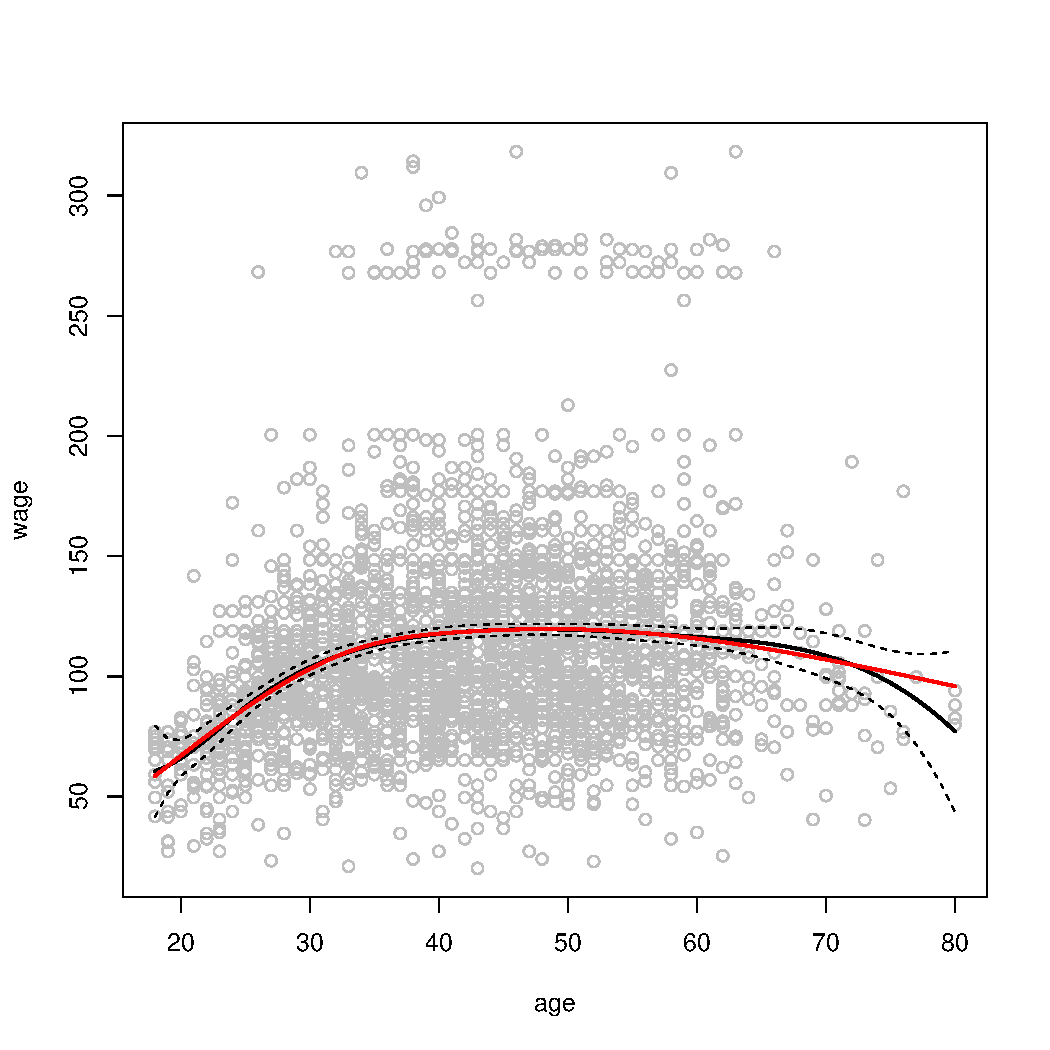
\includegraphics[width=\maxwidth]{figure/unnamed-chunk-20-1} 

\end{knitrout}

As with the \texttt{bs()} function, we could instead specify the knots directly using the \texttt{knots} option.\\

In order to fit a smoothing spline, we use the \texttt{smooth.spline()} function. Recall that the smoothing spline function is minimized by a natural cubic spline with knots at the data points $x_1, \ldots, x_n$. Figure 7.8 was produced with the following code:

\begin{knitrout}
\definecolor{shadecolor}{rgb}{0.969, 0.969, 0.969}\color{fgcolor}\begin{kframe}
\begin{alltt}
\hlkwd{plot}\hlstd{(age, wage,} \hlkwc{xlim}\hlstd{=agelims,} \hlkwc{cex}\hlstd{=}\hlnum{.5}\hlstd{,} \hlkwc{col}\hlstd{=}\hlstr{"darkgrey"}\hlstd{)}
\hlkwd{title}\hlstd{(}\hlstr{"Smoothing Spline"}\hlstd{)}
\hlstd{fit}\hlkwb{=}\hlkwd{smooth.spline}\hlstd{(age, wage,} \hlkwc{df}\hlstd{=}\hlnum{16}\hlstd{)}
\hlstd{fit2}\hlkwb{=}\hlkwd{smooth.spline}\hlstd{(age, wage,} \hlkwc{cv}\hlstd{=}\hlnum{TRUE}\hlstd{)}
\hlstd{fit2}\hlopt{$}\hlstd{df}
\end{alltt}
\begin{verbatim}
## [1] 6.794596
\end{verbatim}
\begin{alltt}
\hlkwd{lines}\hlstd{(fit,} \hlkwc{col}\hlstd{=}\hlstr{"red"}\hlstd{,}\hlkwc{lwd}\hlstd{=}\hlnum{2}\hlstd{)}
\hlkwd{lines}\hlstd{(fit2,}\hlkwc{col}\hlstd{=}\hlstr{"blue"}\hlstd{,}\hlkwc{lwd}\hlstd{=}\hlnum{2}\hlstd{)}
\hlkwd{legend}\hlstd{(}\hlstr{"topright"}\hlstd{,}\hlkwc{legend}\hlstd{=}\hlkwd{c}\hlstd{(}\hlstr{"16 DF"}\hlstd{,} \hlstr{"6.8 DF"}\hlstd{),} \hlkwc{col}\hlstd{=}\hlkwd{c}\hlstd{(}\hlstr{"red"}\hlstd{,}\hlstr{"blue"}\hlstd{),} \hlkwc{lty}\hlstd{=}\hlnum{1}\hlstd{,} \hlkwc{lwd}\hlstd{=}\hlnum{2}\hlstd{,} \hlkwc{cex}\hlstd{=}\hlnum{0.8}\hlstd{)}
\end{alltt}
\end{kframe}
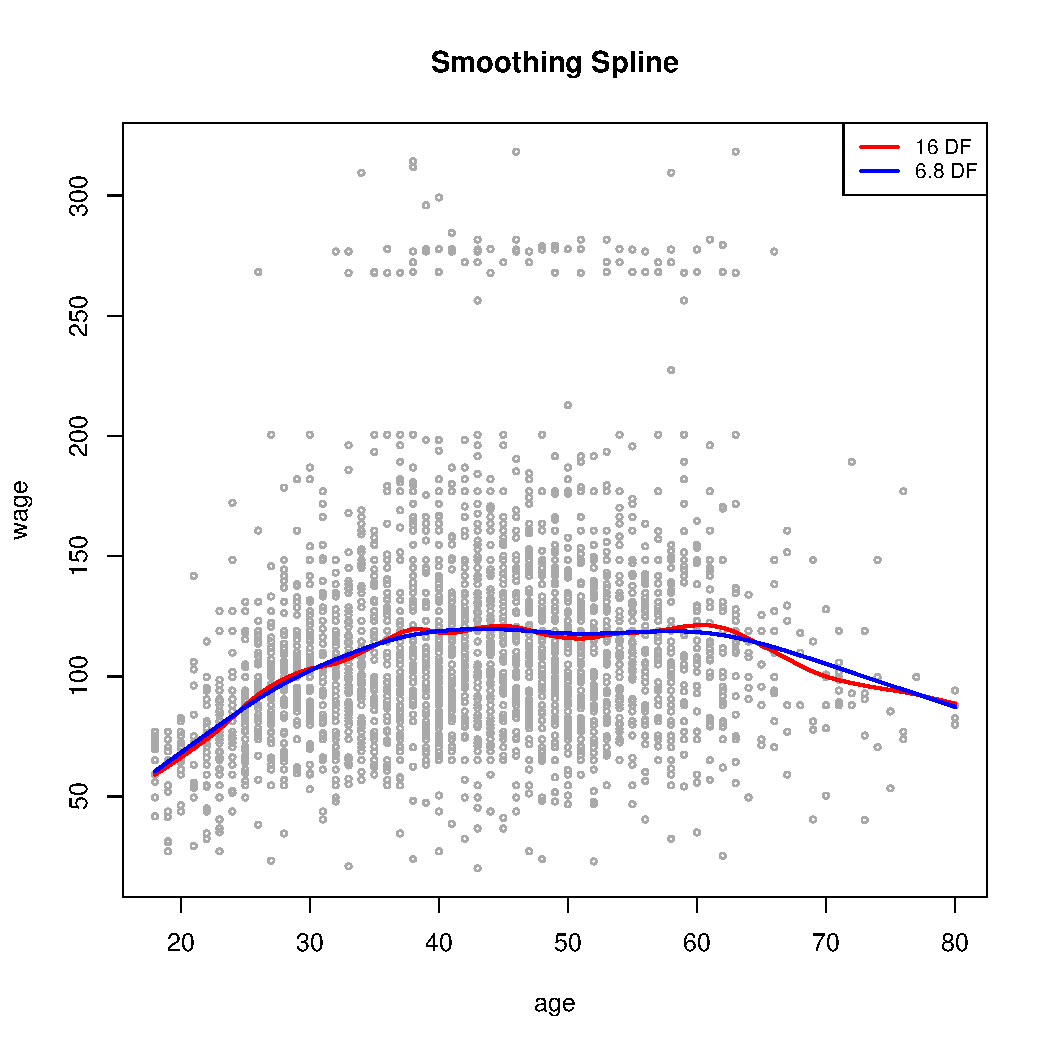
\includegraphics[width=\maxwidth]{figure/unnamed-chunk-21-1} 

\end{knitrout}

Notice in the first call to \texttt{smooth.spline()}, we specified \texttt{df=16}. The function then determines which value of $\lambda$ leads to $16$ degrees of freedom. In the second call to \texttt{smooth.spline()}, we select the smoothness level by cross-validation; this results in a value of $\lambda$ that yields $6.8$ degrees of freedom.\\

In order to perform local regression, we use the \texttt{loess()} function.

\begin{knitrout}
\definecolor{shadecolor}{rgb}{0.969, 0.969, 0.969}\color{fgcolor}\begin{kframe}
\begin{alltt}
\hlkwd{plot}\hlstd{(age, wage,} \hlkwc{xlim}\hlstd{=agelims,} \hlkwc{cex}\hlstd{=}\hlnum{.5}\hlstd{,} \hlkwc{col}\hlstd{=}\hlstr{"darkgrey"}\hlstd{)}
\hlkwd{title}\hlstd{(}\hlstr{"Local Regression"}\hlstd{)}
\hlstd{fit}\hlkwb{=}\hlkwd{loess}\hlstd{(wage}\hlopt{~}\hlstd{age,} \hlkwc{span}\hlstd{=}\hlnum{.2}\hlstd{,} \hlkwc{data}\hlstd{=Wage)}
\hlstd{fit2}\hlkwb{=}\hlkwd{loess}\hlstd{(wage}\hlopt{~}\hlstd{age,} \hlkwc{span}\hlstd{=}\hlnum{.5}\hlstd{,} \hlkwc{data}\hlstd{=Wage)}

\hlkwd{lines}\hlstd{(age.grid,} \hlkwd{predict}\hlstd{(fit,} \hlkwd{data.frame}\hlstd{(}\hlkwc{age}\hlstd{=age.grid)),} \hlkwc{col}\hlstd{=}\hlstr{"red"}\hlstd{,} \hlkwc{lwd}\hlstd{=}\hlnum{2}\hlstd{)}
\hlkwd{lines}\hlstd{(age.grid,} \hlkwd{predict}\hlstd{(fit2,}\hlkwd{data.frame}\hlstd{(}\hlkwc{age}\hlstd{=age.grid)),} \hlkwc{col}\hlstd{=}\hlstr{"blue"}\hlstd{,} \hlkwc{lwd}\hlstd{=}\hlnum{2}\hlstd{)}

\hlkwd{legend}\hlstd{(}\hlstr{"topright"}\hlstd{,} \hlkwc{legend}\hlstd{=}\hlkwd{c}\hlstd{(}\hlstr{"Span=0.2"}\hlstd{,} \hlstr{"Span=0.5"}\hlstd{),}
       \hlkwc{col}\hlstd{=}\hlkwd{c}\hlstd{(}\hlstr{"red"}\hlstd{,}\hlstr{"blue"}\hlstd{),} \hlkwc{lty}\hlstd{=}\hlnum{1}\hlstd{,} \hlkwc{lwd}\hlstd{=}\hlnum{2}\hlstd{,} \hlkwc{cex}\hlstd{=}\hlnum{.8}\hlstd{)}
\end{alltt}
\end{kframe}
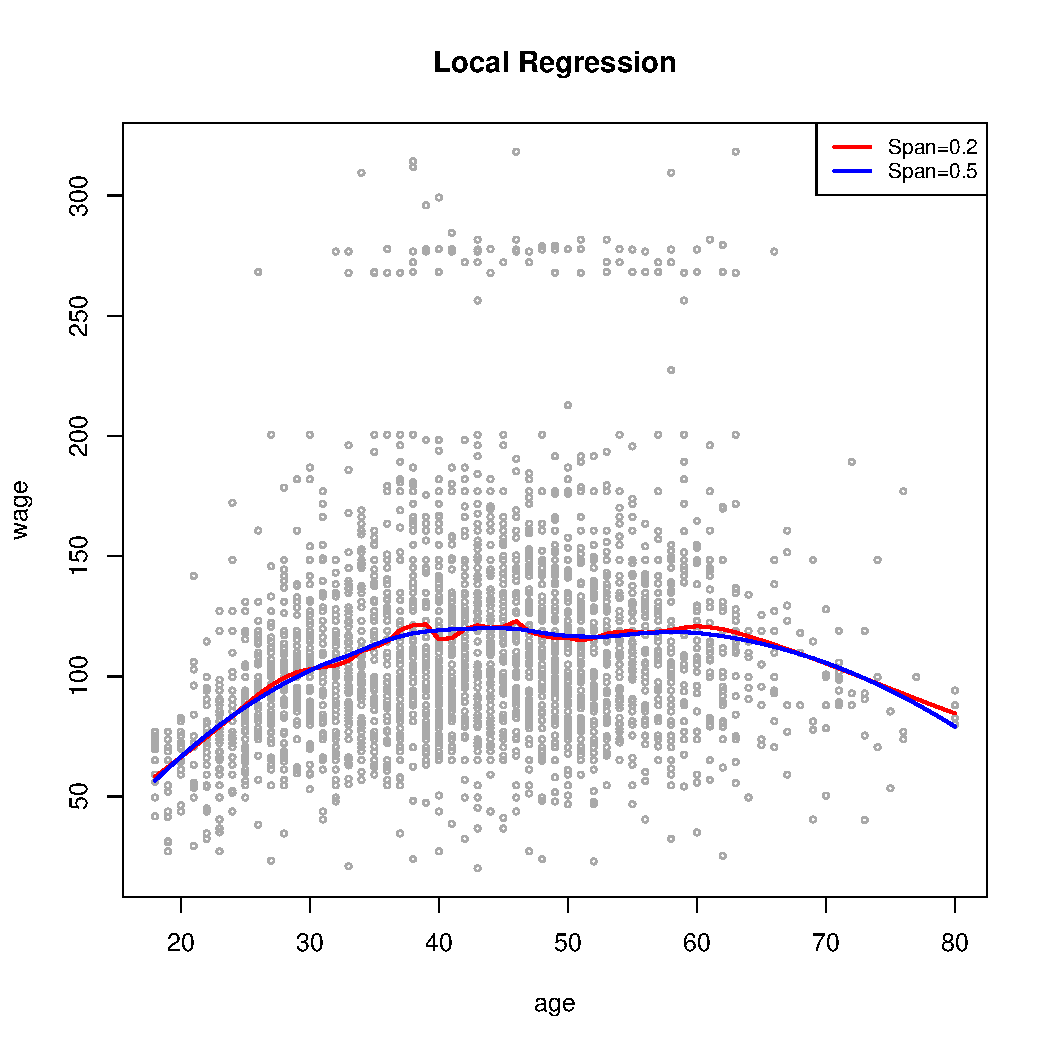
\includegraphics[width=\maxwidth]{figure/unnamed-chunk-22-1} 

\end{knitrout}


Here we have performed local linear regression using spans of 0.2 and 0.5. That is, each neighborhood consists of 20\% or 50\% of the observations. The larger the span, the smoother the fit. The \texttt{locfit} library can also be used for fitting local regression models in \texttt{R}.

\section{GAMs}

We now fit a GAM to predict \texttt{wage} using natural spline functions of \texttt{year} and \texttt{age}, treating \texttt{education} as a qualitative predictor as in (7.16). Since this is just a big linear regression model using an appropriate choice of basis functions, we can simply do this using the \texttt{lm()} function.

\begin{knitrout}
\definecolor{shadecolor}{rgb}{0.969, 0.969, 0.969}\color{fgcolor}\begin{kframe}
\begin{alltt}
\hlstd{gam1} \hlkwb{=} \hlkwd{lm}\hlstd{(wage}\hlopt{~}\hlkwd{ns}\hlstd{(year,}\hlnum{4}\hlstd{)} \hlopt{+} \hlkwd{ns}\hlstd{(age,}\hlnum{5}\hlstd{)} \hlopt{+} \hlstd{education,} \hlkwc{data} \hlstd{= Wage)}
\end{alltt}
\end{kframe}
\end{knitrout}

We now fit the model (7.16) using smoothing splines rather than natural splines. In order to fit more general sorts of GAMs, using smoothing splines or other components that cannot be expressed in terms of basis functions and then fit using least squares regression, we will need to use the \texttt{gam} library in \texttt{R}.\\

The \texttt{s()} function, which is part of the \texttt{gam} library, is used to indicate that we would like to use a smoothing spline. We specify that the function of \texttt{year} should have 4 degrees of freedom, and that the function of \texttt{age} will have 5 degrees of freedom. Since \texttt{education} is qualitative, we leave it as is and it is converted into four dummy variables. We use the \texttt{gam()} function in order to fit a GAM using these components. All of the terms in (7.16) are fit simultaneously, taking each other into account to explain the response.

\begin{knitrout}
\definecolor{shadecolor}{rgb}{0.969, 0.969, 0.969}\color{fgcolor}\begin{kframe}
\begin{alltt}
\hlstd{gam.m3} \hlkwb{=} \hlkwd{gam}\hlstd{(wage}\hlopt{~}\hlkwd{s}\hlstd{(year,}\hlnum{4}\hlstd{)} \hlopt{+} \hlkwd{s}\hlstd{(age,}\hlnum{5}\hlstd{)} \hlopt{+} \hlstd{education,} \hlkwc{data}\hlstd{=Wage)}
\end{alltt}
\end{kframe}
\end{knitrout}

In order to produce Figure 7.12, we simply call the \texttt{plot()} function:

\begin{knitrout}
\definecolor{shadecolor}{rgb}{0.969, 0.969, 0.969}\color{fgcolor}\begin{kframe}
\begin{alltt}
\hlkwd{par}\hlstd{(}\hlkwc{mfrow}\hlstd{=}\hlkwd{c}\hlstd{(}\hlnum{1}\hlstd{,}\hlnum{3}\hlstd{))}
\hlkwd{plot}\hlstd{(gam.m3,} \hlkwc{se}\hlstd{=}\hlnum{TRUE}\hlstd{,} \hlkwc{col}\hlstd{=}\hlstr{"blue"}\hlstd{)}
\end{alltt}
\end{kframe}
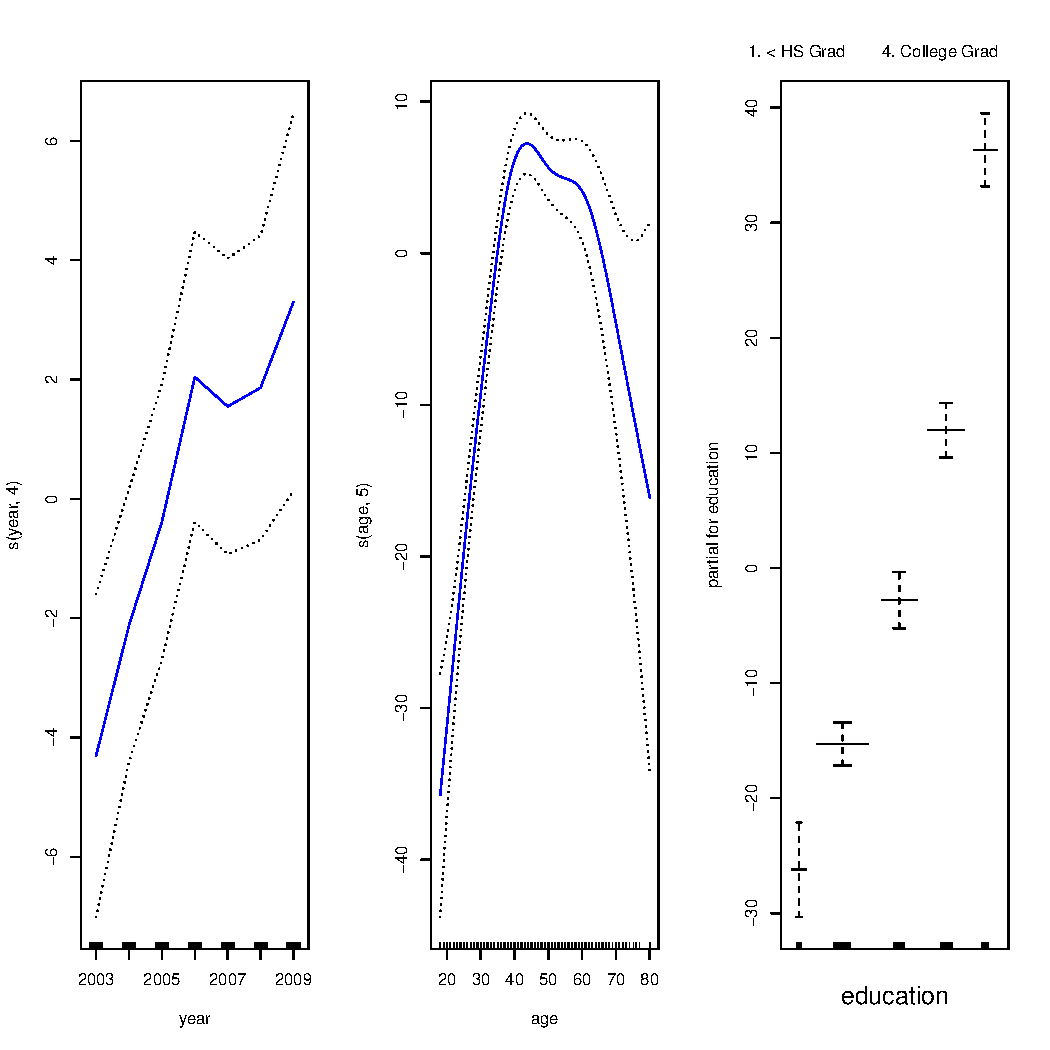
\includegraphics[width=\maxwidth]{figure/unnamed-chunk-25-1} 

\end{knitrout}

The generic \texttt{plot()} function recognizes that \texttt{gam.m3} is an object of class \texttt{gam}, and invokes the appropriate \texttt{plot.Gam()} method. Conveniently, even though \texttt{gam1} is not of class \texttt{gam} but rather of class \texttt{lm}, we can still use \texttt{plot.Gam()} on it. Figure 7.11 was produced using the following expression:

\begin{knitrout}
\definecolor{shadecolor}{rgb}{0.969, 0.969, 0.969}\color{fgcolor}\begin{kframe}
\begin{alltt}
\hlkwd{par}\hlstd{(}\hlkwc{mfrow}\hlstd{=}\hlkwd{c}\hlstd{(}\hlnum{1}\hlstd{,}\hlnum{3}\hlstd{))}

\hlkwd{plot.Gam}\hlstd{(gam1,} \hlkwc{se}\hlstd{=}\hlnum{TRUE}\hlstd{,} \hlkwc{col}\hlstd{=}\hlstr{"red"}\hlstd{)}
\end{alltt}
\end{kframe}
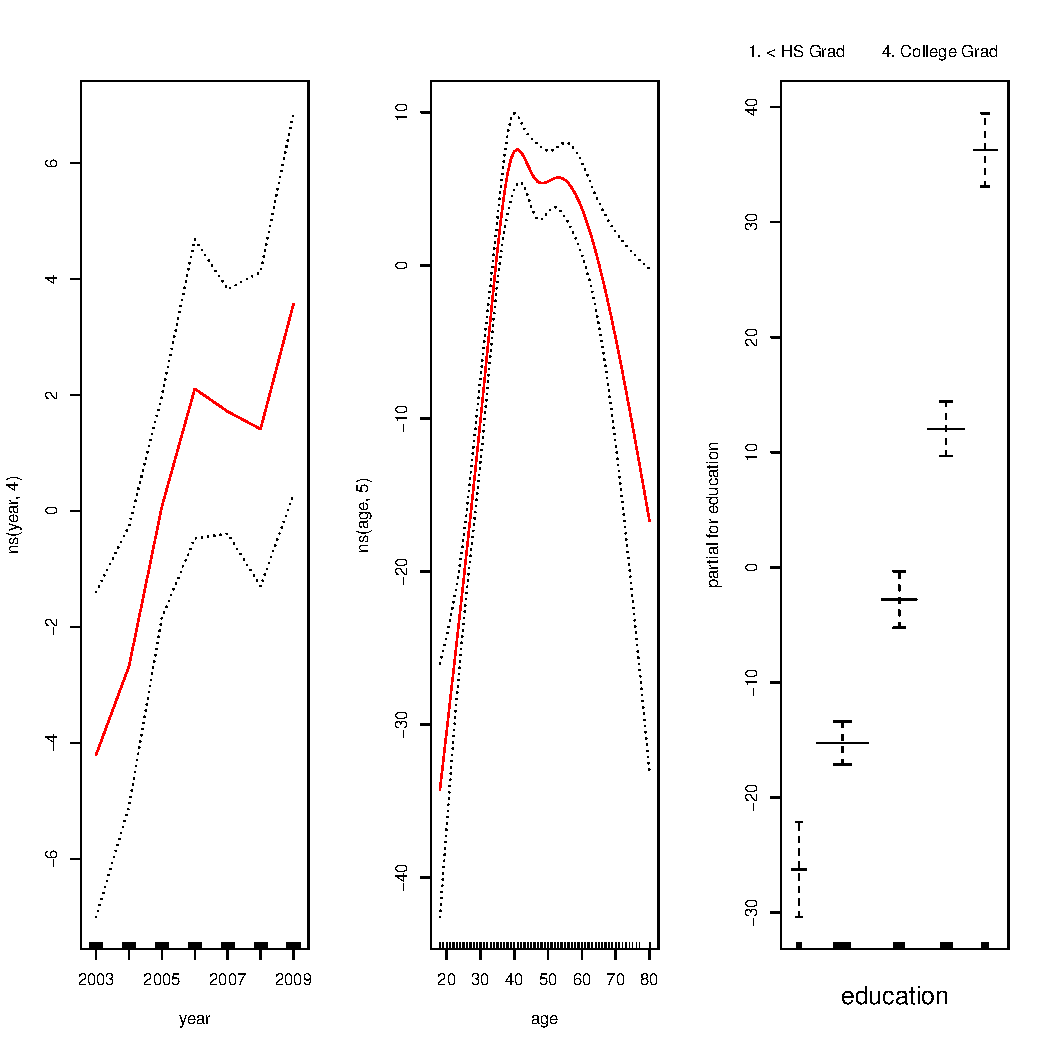
\includegraphics[width=\maxwidth]{figure/unnamed-chunk-26-1} 

\end{knitrout}

Notice here we had to use \texttt{plot.Gam()} rather than the generic \texttt{plot()} function.\\

In these plots, the function of \texttt{year} looks rather linear. We can perform a series of ANOVA tests in order to determine which of these three models is best: a GAM that excludes \texttt{year} ($M_1$), a GAM that uses a linear function of \texttt{year} ($M_2$), or a GAM that uses a spline function of year ($M_3$).

\begin{knitrout}
\definecolor{shadecolor}{rgb}{0.969, 0.969, 0.969}\color{fgcolor}\begin{kframe}
\begin{alltt}
\hlstd{gam.m1}\hlkwb{=}\hlkwd{gam}\hlstd{(wage}\hlopt{~}\hlkwd{s}\hlstd{(age,}\hlnum{5}\hlstd{)}\hlopt{+}\hlstd{education,} \hlkwc{data}\hlstd{=Wage)}
\hlstd{gam.m2}\hlkwb{=}\hlkwd{gam}\hlstd{(wage}\hlopt{~}\hlstd{year}\hlopt{+}\hlkwd{s}\hlstd{(age,}\hlnum{5}\hlstd{)}\hlopt{+}\hlstd{education,} \hlkwc{data}\hlstd{=Wage)}
\hlkwd{anova}\hlstd{(gam.m1, gam.m2, gam.m3,} \hlkwc{test}\hlstd{=}\hlstr{"F"}\hlstd{)}
\end{alltt}
\begin{verbatim}
## Analysis of Deviance Table
## 
## Model 1: wage ~ s(age, 5) + education
## Model 2: wage ~ year + s(age, 5) + education
## Model 3: wage ~ s(year, 4) + s(age, 5) + education
##   Resid. Df Resid. Dev Df Deviance       F    Pr(>F)    
## 1      2990    3711731                                  
## 2      2989    3693842  1  17889.2 14.4771 0.0001447 ***
## 3      2986    3689770  3   4071.1  1.0982 0.3485661    
## ---
## Signif. codes:  0 '***' 0.001 '**' 0.01 '*' 0.05 '.' 0.1 ' ' 1
\end{verbatim}
\end{kframe}
\end{knitrout}

We find that there is compelling evidence that a GAM with a linear function of \texttt{year} is better than a GAM that does not include \texttt{year} at all. However, there is no evidence that a non-linear function of \texttt{year} is needed. In other words, based on the results of this ANOVA, $M_2$ is preferred.\\

The \texttt{summary()} function produces a summary of the gam fit.

\begin{knitrout}
\definecolor{shadecolor}{rgb}{0.969, 0.969, 0.969}\color{fgcolor}\begin{kframe}
\begin{alltt}
\hlkwd{summary}\hlstd{(gam.m3)}
\end{alltt}
\begin{verbatim}
## 
## Call: gam(formula = wage ~ s(year, 4) + s(age, 5) + education, data = Wage)
## Deviance Residuals:
##     Min      1Q  Median      3Q     Max 
## -119.43  -19.70   -3.33   14.17  213.48 
## 
## (Dispersion Parameter for gaussian family taken to be 1235.69)
## 
##     Null Deviance: 5222086 on 2999 degrees of freedom
## Residual Deviance: 3689770 on 2986 degrees of freedom
## AIC: 29887.75 
## 
## Number of Local Scoring Iterations: NA 
## 
## Anova for Parametric Effects
##              Df  Sum Sq Mean Sq F value    Pr(>F)    
## s(year, 4)    1   27162   27162  21.981 2.877e-06 ***
## s(age, 5)     1  195338  195338 158.081 < 2.2e-16 ***
## education     4 1069726  267432 216.423 < 2.2e-16 ***
## Residuals  2986 3689770    1236                      
## ---
## Signif. codes:  0 '***' 0.001 '**' 0.01 '*' 0.05 '.' 0.1 ' ' 1
## 
## Anova for Nonparametric Effects
##             Npar Df Npar F  Pr(F)    
## (Intercept)                          
## s(year, 4)        3  1.086 0.3537    
## s(age, 5)         4 32.380 <2e-16 ***
## education                            
## ---
## Signif. codes:  0 '***' 0.001 '**' 0.01 '*' 0.05 '.' 0.1 ' ' 1
\end{verbatim}
\end{kframe}
\end{knitrout}

The p-values for \texttt{year} and \texttt{age} correspond to a null hypothesis of a linear relationship versus the alternative of a non-linear relationship. The large p-value for \texttt{year} reinforces our conclusion from the ANOVA test that a linear function is adequate for this term. However, there is very clear evidence that a non-linear term is required for \texttt{age}.\\

We can make predictions from \texttt{gam} objects, just like from \texttt{lm} objects, using the \texttt{predict()} method for the class \texttt{gam}. Here we make predictions on the training set.

\begin{knitrout}
\definecolor{shadecolor}{rgb}{0.969, 0.969, 0.969}\color{fgcolor}\begin{kframe}
\begin{alltt}
\hlstd{preds} \hlkwb{=} \hlkwd{predict}\hlstd{(gam.m2,} \hlkwc{newdata}\hlstd{=Wage)}
\end{alltt}
\end{kframe}
\end{knitrout}

We can also use local regression fits as building blocks in a GAM, using the \texttt{lo()} function.

\begin{knitrout}
\definecolor{shadecolor}{rgb}{0.969, 0.969, 0.969}\color{fgcolor}\begin{kframe}
\begin{alltt}
\hlkwd{par}\hlstd{(}\hlkwc{mfrow}\hlstd{=}\hlkwd{c}\hlstd{(}\hlnum{1}\hlstd{,}\hlnum{3}\hlstd{))}

\hlstd{gam.lo} \hlkwb{=} \hlkwd{gam}\hlstd{(wage}\hlopt{~}\hlkwd{s}\hlstd{(year,} \hlkwc{df} \hlstd{=}\hlnum{4}\hlstd{)}\hlopt{+} \hlkwd{lo}\hlstd{(age,} \hlkwc{span}\hlstd{=}\hlnum{0.7}\hlstd{)} \hlopt{+} \hlstd{education,}
             \hlkwc{data}\hlstd{=Wage)}
\hlkwd{plot.Gam}\hlstd{(gam.lo,} \hlkwc{set}\hlstd{=}\hlnum{TRUE}\hlstd{,} \hlkwc{col}\hlstd{=}\hlstr{"green"}\hlstd{)}
\end{alltt}
\end{kframe}
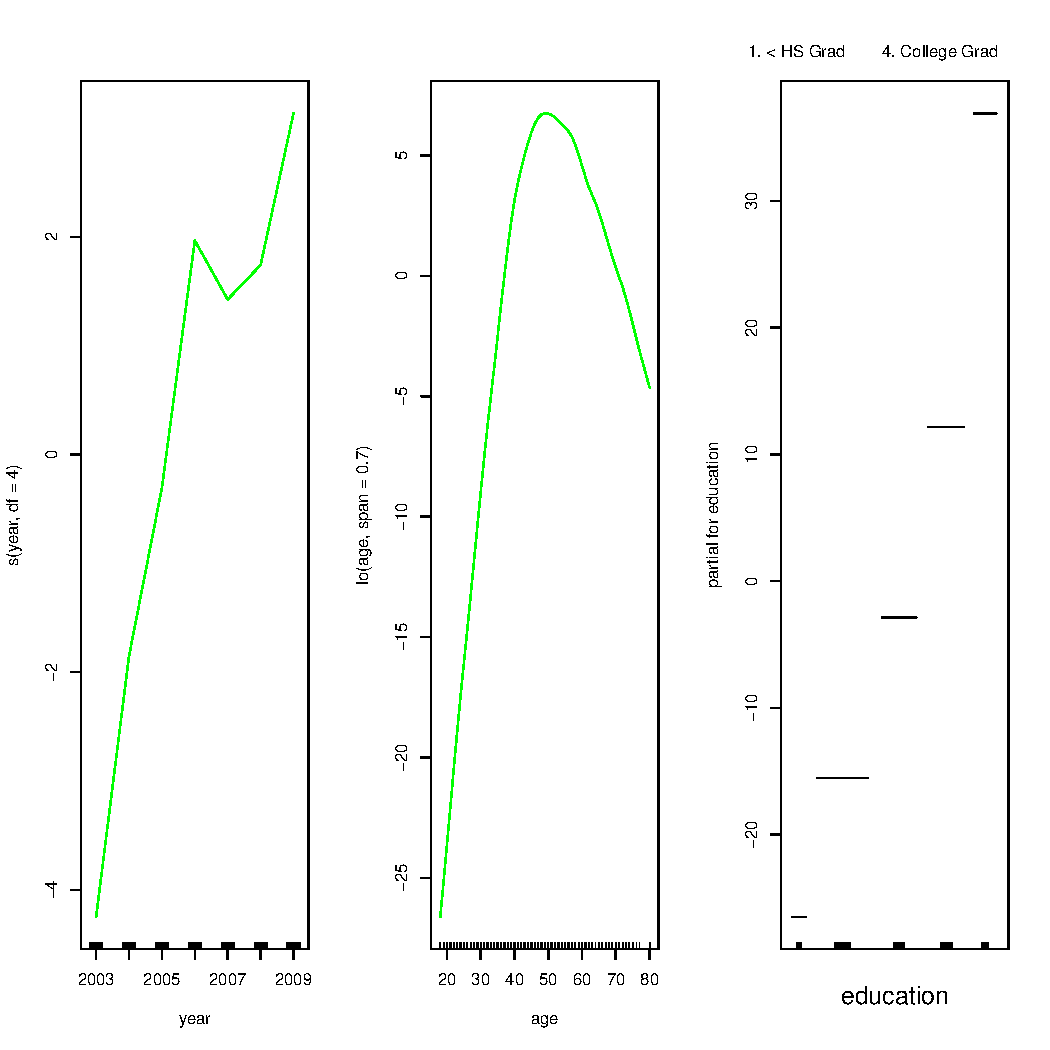
\includegraphics[width=\maxwidth]{figure/unnamed-chunk-30-1} 

\end{knitrout}

Here we have used local regression for the \texttt{age} term, with a span of 0.7. We can also use the \texttt{lo()} function to create interactions before calling the \texttt{gam()} function. For example,

\begin{knitrout}
\definecolor{shadecolor}{rgb}{0.969, 0.969, 0.969}\color{fgcolor}\begin{kframe}
\begin{alltt}
\hlstd{gam.lo.i} \hlkwb{=} \hlkwd{gam}\hlstd{(wage}\hlopt{~}\hlkwd{lo}\hlstd{(year, age,} \hlkwc{span}\hlstd{=}\hlnum{0.5}\hlstd{)}\hlopt{+}\hlstd{education,} \hlkwc{data}\hlstd{=Wage)}
\end{alltt}
\end{kframe}
\end{knitrout}

fits a two-term model, in which the first term is an interaction between \texttt{year} and \texttt{age}, fit by a local regression surface. We can plot the resulting two-dimensional surface if we first install the \texttt{akima} package.

\begin{knitrout}
\definecolor{shadecolor}{rgb}{0.969, 0.969, 0.969}\color{fgcolor}\begin{kframe}
\begin{alltt}
\hlkwd{par}\hlstd{(}\hlkwc{mfrow}\hlstd{=}\hlkwd{c}\hlstd{(}\hlnum{1}\hlstd{,}\hlnum{3}\hlstd{))}

\hlkwd{plot}\hlstd{(gam.lo.i)}
\end{alltt}
\end{kframe}
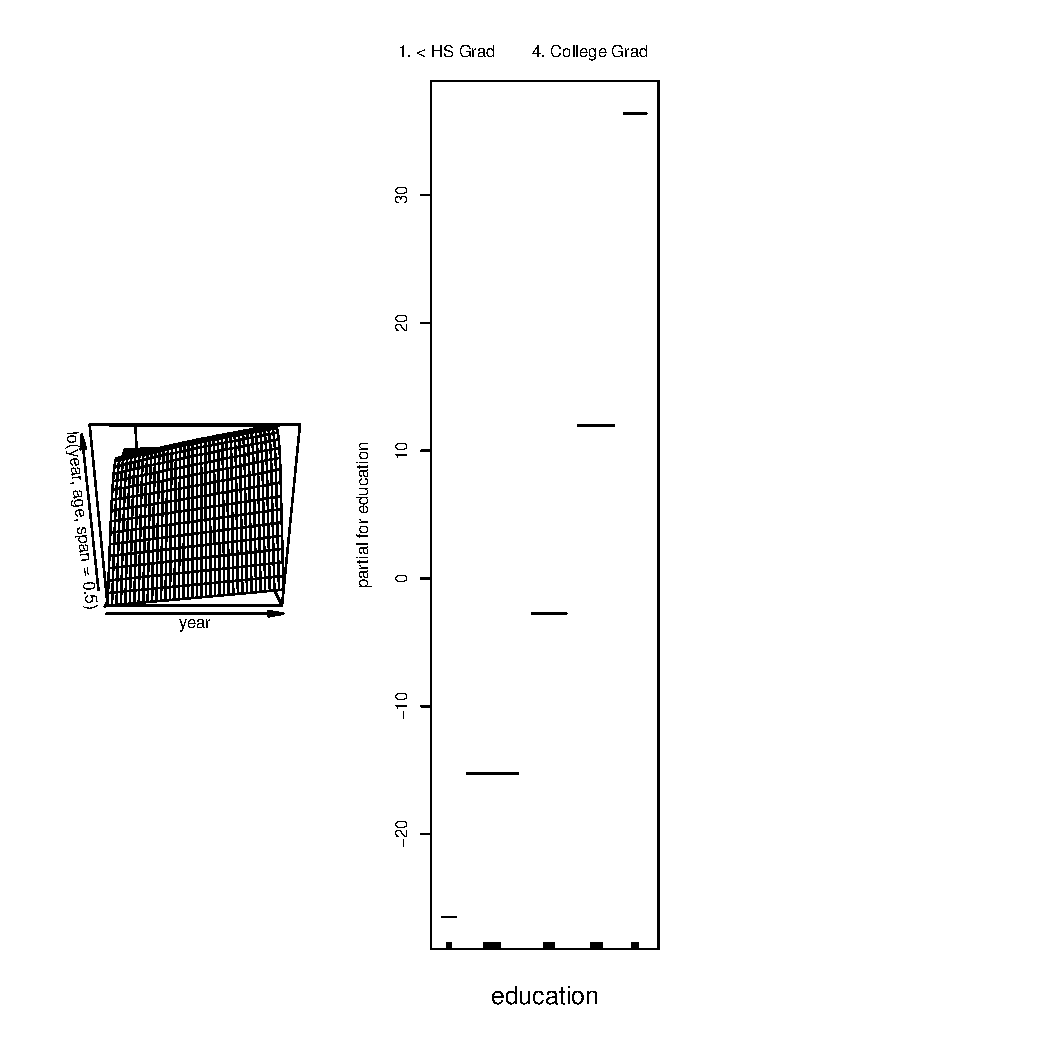
\includegraphics[width=\maxwidth]{figure/unnamed-chunk-32-1} 

\end{knitrout}

In order to fit a logistic regression GAM, we once again use the \texttt{I()} function in constructing the binary response variable, and set \texttt{family = binomial}.

\begin{knitrout}
\definecolor{shadecolor}{rgb}{0.969, 0.969, 0.969}\color{fgcolor}\begin{kframe}
\begin{alltt}
\hlkwd{par}\hlstd{(}\hlkwc{mfrow}\hlstd{=}\hlkwd{c}\hlstd{(}\hlnum{1}\hlstd{,}\hlnum{3}\hlstd{))}

\hlstd{gam.lr}\hlkwb{=}\hlkwd{gam}\hlstd{(}\hlkwd{I}\hlstd{(wage}\hlopt{>}\hlnum{250}\hlstd{)}\hlopt{~}\hlstd{year}\hlopt{+}\hlkwd{s}\hlstd{(age,}\hlkwc{df}\hlstd{=}\hlnum{5}\hlstd{)}\hlopt{+}\hlstd{education,}
           \hlkwc{family} \hlstd{= binomial,} \hlkwc{data} \hlstd{= Wage)}
\hlkwd{par}\hlstd{(}\hlkwc{mfrow}\hlstd{=}\hlkwd{c}\hlstd{(}\hlnum{1}\hlstd{,}\hlnum{3}\hlstd{))}
\hlkwd{plot}\hlstd{(gam.lr,} \hlkwc{se}\hlstd{=T,} \hlkwc{col}\hlstd{=}\hlstr{"green"}\hlstd{)}
\end{alltt}
\end{kframe}
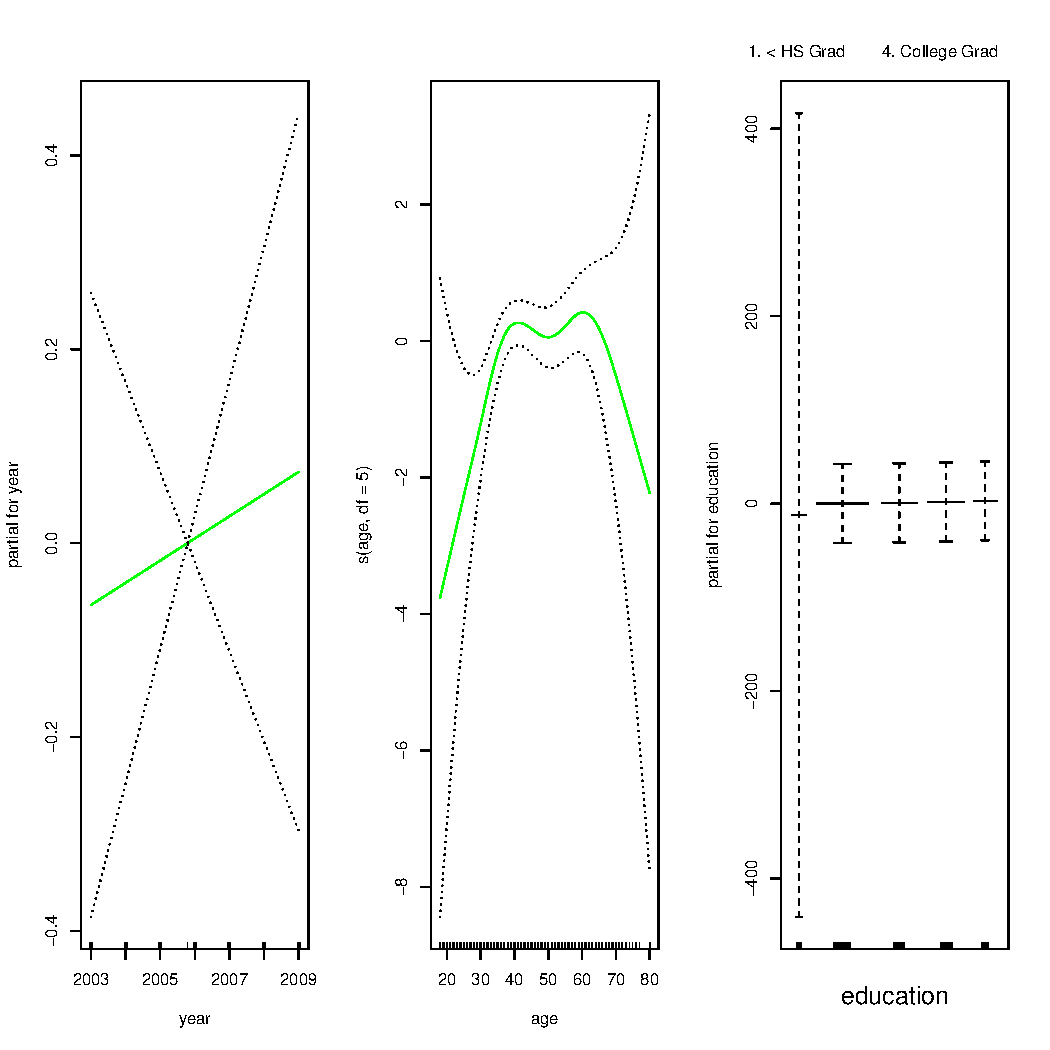
\includegraphics[width=\maxwidth]{figure/unnamed-chunk-33-1} 

\end{knitrout}

It is easy to see that there are no high earners in the \texttt{<HS} category:

\begin{knitrout}
\definecolor{shadecolor}{rgb}{0.969, 0.969, 0.969}\color{fgcolor}\begin{kframe}
\begin{alltt}
\hlkwd{table}\hlstd{(education,} \hlkwd{I}\hlstd{(wage}\hlopt{>}\hlnum{250}\hlstd{))}
\end{alltt}
\begin{verbatim}
##                     
## education            FALSE TRUE
##   1. < HS Grad         268    0
##   2. HS Grad           966    5
##   3. Some College      643    7
##   4. College Grad      663   22
##   5. Advanced Degree   381   45
\end{verbatim}
\end{kframe}
\end{knitrout}

Hence, we git a logistic regression GAM using all but this category. This provides more sensible results.

\begin{knitrout}
\definecolor{shadecolor}{rgb}{0.969, 0.969, 0.969}\color{fgcolor}\begin{kframe}
\begin{alltt}
\hlkwd{par}\hlstd{(}\hlkwc{mfrow}\hlstd{=}\hlkwd{c}\hlstd{(}\hlnum{1}\hlstd{,}\hlnum{3}\hlstd{))}

\hlstd{gam.lr.s} \hlkwb{=} \hlkwd{gam}\hlstd{(}\hlkwd{I}\hlstd{(wage}\hlopt{>}\hlnum{250}\hlstd{)}\hlopt{~}\hlstd{year}\hlopt{+}\hlkwd{s}\hlstd{(age,} \hlkwc{df}\hlstd{=}\hlnum{5}\hlstd{)}\hlopt{+}\hlstd{education,}
               \hlkwc{family}\hlstd{=binomial,} \hlkwc{data}\hlstd{=Wage,}
               \hlkwc{subset}\hlstd{=(education}\hlopt{!=}\hlstr{"1. < HS Grad"}\hlstd{))}
\hlkwd{plot}\hlstd{(gam.lr.s,} \hlkwc{se}\hlstd{=T,} \hlkwc{col}\hlstd{=}\hlstr{"green"}\hlstd{)}
\end{alltt}
\end{kframe}
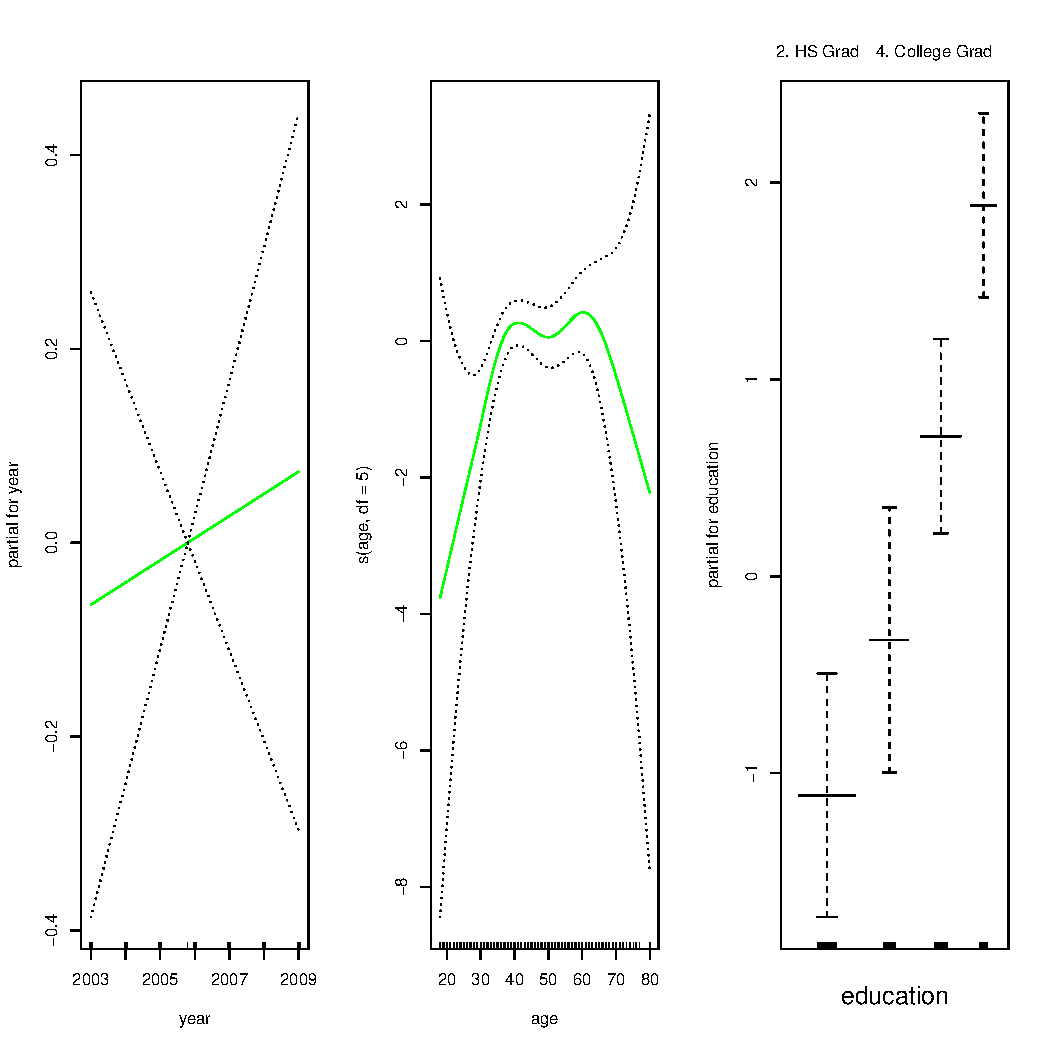
\includegraphics[width=\maxwidth]{figure/unnamed-chunk-35-1} 

\end{knitrout}


\end{document}
